

\chapter{Linear Regression}

	\section{Simple Linear Regression}
		We assume the following relationship among the data
		\begin{center}
			$Y \approx \beta_0 + \beta_1X$
		\end{center}
		We regress $Y$ on (onto) $X$
		\begin{center}
			$sales \approx \beta_0 + \beta_1 \times TV$
		\end{center}
		This is a simple \textbf{unvariate model}.
		$\beta_0$, intercept, and $\beta_1$ slope, both are \textbf{coefficients} or \textbf{parameters}.\\
		The estimated value of $Y$ on input $X=x$ is denoted by
		\begin{center}
			$\hat{y} = \hat{\beta}_0 + \hat{\beta}_1 x$
		\end{center}
		\textbf{Given} training data set of $n$ observations
		\begin{center}
			$(x_1,y_1),(x_3,y_2),...,(x_n,y_n)$
		\end{center}
		\textbf{Goal} estimate the unknown coefficients $\beta_0$ and $\beta_1$ such that
		\begin{center}
			$y_i \approx \hat{\beta}_0 + \hat{\beta}_1 x_i$
		\end{center}
		for all $i=1,...,n$ and for future values of $x$.
	
	
	\section{Estimating the Coefficients}
		We We measure deviation of the estimate to the true value by a \textbf{loss function}.
		We mostly use the \textbf{least-squares} function for this purpose.\\
		Let $\hat{y}_i = \hat{\beta}_0 + \hat{\beta}_1 x_i$, then $e_i = y_i - \hat{y}_i$ is the 
		\textbf{residual sum of squares (RSS)}
		\begin{align*}
			RSS &:= e^2_1 + e^2_2 + ... + e^2_n\\
			&= (y_1 - \hat{\beta}_0 + \hat{\beta}_1 x_1)^2 + (y_2 - \hat{\beta}_0 + \hat{\beta}_1 x_2)^2
			+ ... + (y_n - \hat{\beta}_0 + \hat{\beta}_1 x_n)^2
		\end{align*}
		This is a quadratic function in $\beta_0$ and $\beta_1$.
		Setting its derivative to zero yields the least-square coefficient estimates.
		\begin{center}
			$\hat{\beta}_1 = \frac{\sum\limits_{i=1}^m (x_i-\bar{x})(y_i-\bar{y})}{\sum\limits_{i=1}^m (x_i-\bar{x})^2}$
			\ \ \ \ \ \ and\ \ \ \ \ \ 
			$\hat{\beta}_0 = \bar{y} - \hat{\beta}_1\bar{x}$
		\end{center}
		with
		\begin{center}
			\ \ \ \ \ \ \ \ \ 
			$\hat{x} = \frac{1}{n} \sum\limits_{i=1}^n x_i$
			\ \ \ \ \ \ and\ \ \ \ \ \ 
			$\hat{y} = \frac{1}{n} \sum\limits_{i=1}^n y_i$.
		\end{center}
		
		\begin{figure}[ht]
			\centering
			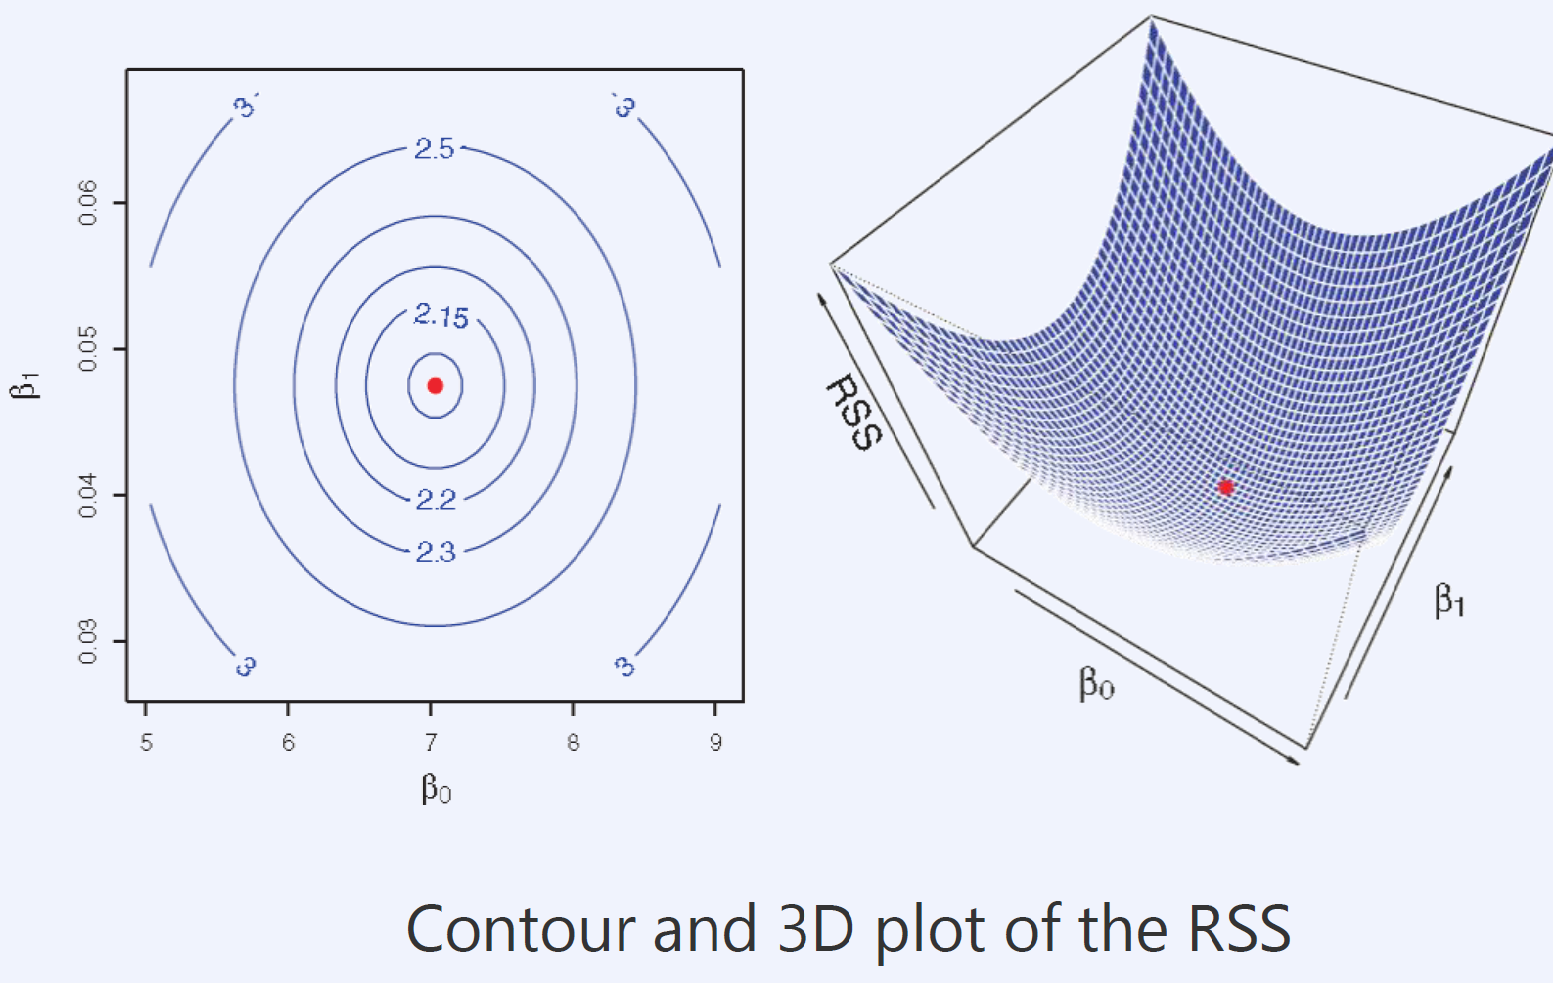
\includegraphics[width=1\linewidth]{Graphics/LinearRegression/1.png}
			\caption{Contour and 3D plot of the RSS}
		\end{figure}
	
	
	\section{Accuracy of Coefficient Estimates}
		We assume the true relationship has an additional noise component that is independent from observations
		\begin{center}
			$Y = \beta_0 + \beta_1X + \epsilon$\ \ \ (*)
		\end{center}
		This is the \textbf{population regression line}, the best linear approximation to the true relationship between $X$ and $Y$, given that the true relationship is (*).
		The population regression line is usually unobserved.\\
		The least-squares fit on the trining data is given by $\hat{y} = \hat{\beta}_0 + \hat{\beta}_1x$.
		\begin{figure}[ht]
		  \centering
		  \subfloat[][]{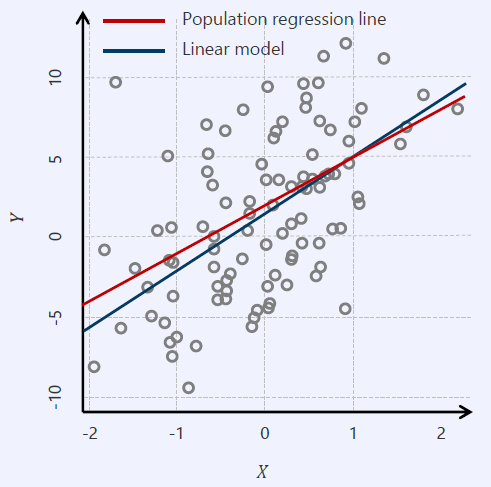
\includegraphics[width=0.4\linewidth]{Graphics/LinearRegression/2.png}}
		  \qquad
		  \subfloat[][]{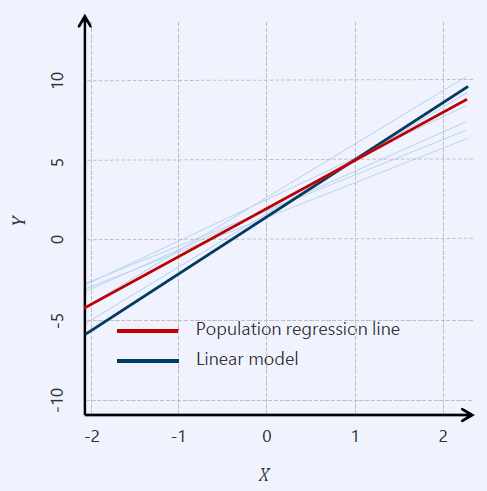
\includegraphics[width=0.4\linewidth]{Graphics/LinearRegression/3.png}}
		\end{figure}
		For example on figure (a) we see Population regression line (red) and least squares fit (blue) on simulated data $𝑌=2+3𝑋+\epsilon$ with Gaussian error $\epsilon$ with $0$ mean.\\
		And on figure (b) we see Ten least squares fits on different randomly chosen training data sets.
	
	
	\section{Unbiased Estimates}
		How do we estimate the mean $\mu$ of a random variable $Y$?
		\begin{itemize}
			\item the sample estimate over a finite set of observations is the average
				\begin{center}
					$Ave(y_1,y_2,...,y_n) = \frac{1}{n} \sum\limits_{i=1}^n y_i = \bar{y}$
				\end{center}
			\item on average, we have $\bar{y}=\mu$. $\bar{y}$ is an unbiased estimate for $\mu$
		\end{itemize}
		In same fashion, \textbf{the least-square fit is an unbiased estimate for the population regression line}!
		\begin{itemize}
			\item furthermore, among all unbiased linear estimators, the least square fit is the one with the smallest variance (\textbf{Gauss Markov Theorem})
		\end{itemize}
	
	
		\subsection{Assessing the Accuracy of Estimates}
			The \textbf{standard error} of $\mu$ is
			\begin{center}
				$SE(\mu) = \sqrt{Var(\mu)} = \sqrt{\frac{\sigma^2}{n}}$
			\end{center}
			\begin{itemize}
				\item $\sigma$ population standard deviation
				item $n$ sample size
			\end{itemize}
			We assume (as we usually do) that all observations are independent.\\
			The \textbf{more} observations we have, the \textbf{smaller} the standard error.\\
			The standard errors of the least-square coefficients are
			\begin{center}
				$SE(\hat{\beta_0})^2 = \sigma^2 \left[\frac{1}{n} + \frac{\bar{x}^2}{\sum\limits_{i=1}^n (x_i - \bar{x})^2}\right]$\\
				$SE(\hat{\beta_1})^2 = \frac{\sigma^2}{\sum\limits_{i=1}^n (x_i - \bar{x})^2}$
			\end{center}
			where $\sigma^2 = Var[\epsilon]$.\\
			Again we assume (mostly incorrectly) that errors are independent and uncorrelated, with the common variance $\sigma^2$.\\\\
			\textbf{Observations}
			\begin{enumerate}
				\item $SE(\hat{\beta}_1)$ decreases as the $x_i$ are more spread out - the slope is easier to determine.
				\item $SE(\hat{\beta}_0) = SE(\hat{\mu})$ if $\bar{x} = 0$ in which case $\hat{\beta}_0 = \bar{y}$.
				\item $\sigma$ is not known but we can provide a sample estimate for it, the residual standard error
					\begin{center}
						$RSE = \sqrt{\frac{RSS}{(n-2)}}$
					\end{center}
			\end{enumerate}
			
\newpage

		\section{Computing Confidence Intervals}
			$95\%$ \textbf{confidence interval}
			\begin{itemize}
				\item interval that will contain the true value with $95\%$ probability
				\item limits are computed from the sample (training) data
			\end{itemize}
			For the linear regression coefficient $\hat{\beta}_1$ it takes approximately the form
			\begin{center}
				$[\hat{\beta}_1 - 2\cdot SE(\hat{\beta}_1)\ ,\ \hat{\beta}_1 + 2 \cdot SE(\hat{\beta}_1)]$
			\end{center}
			analogously for $\hat{\beta}_0$
			\begin{center}
				$[\hat{\beta}_0 - 2\cdot SE(\hat{\beta}_0)\ ,\ \hat{\beta}_0 + 2 \cdot SE(\hat{\beta}_0)]$
			\end{center}
			\textbf{Why} is this the case? (ESL)
			\begin{itemize}
				\item we assume that the error in the output is Gaussian distributed
				\item the coefficient estimates are then also Gaussian distributed (!)
			\end{itemize}
			
			\begin{figure}[ht]
				\centering
				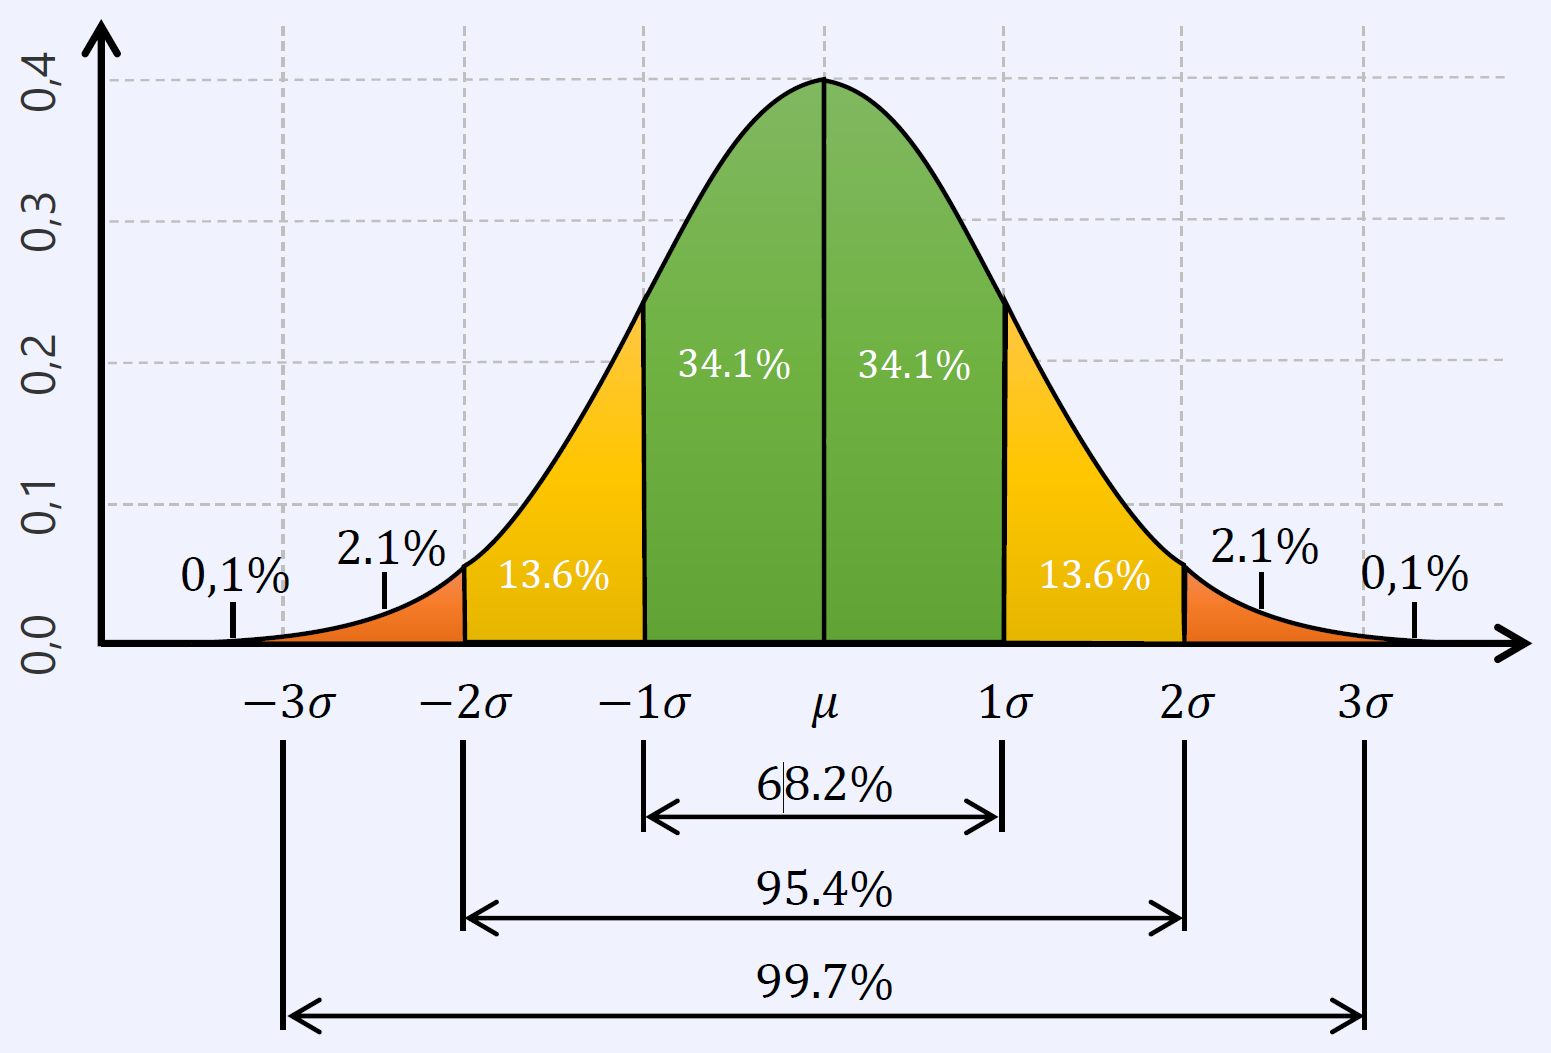
\includegraphics[width=1\linewidth]{Graphics/LinearRegression/4.png}
				\caption{Probability mass in a Gaussian}
			\end{figure}






























